\documentclass{beamer}
\usetheme{default}

\title{Analyzing the evolution of the European Parliament Social Network}

\date{2023-11-10}

\author{Á. Bernát, M. Marits}

\usepackage{graphicx}

%\setbeamertemplate{background}{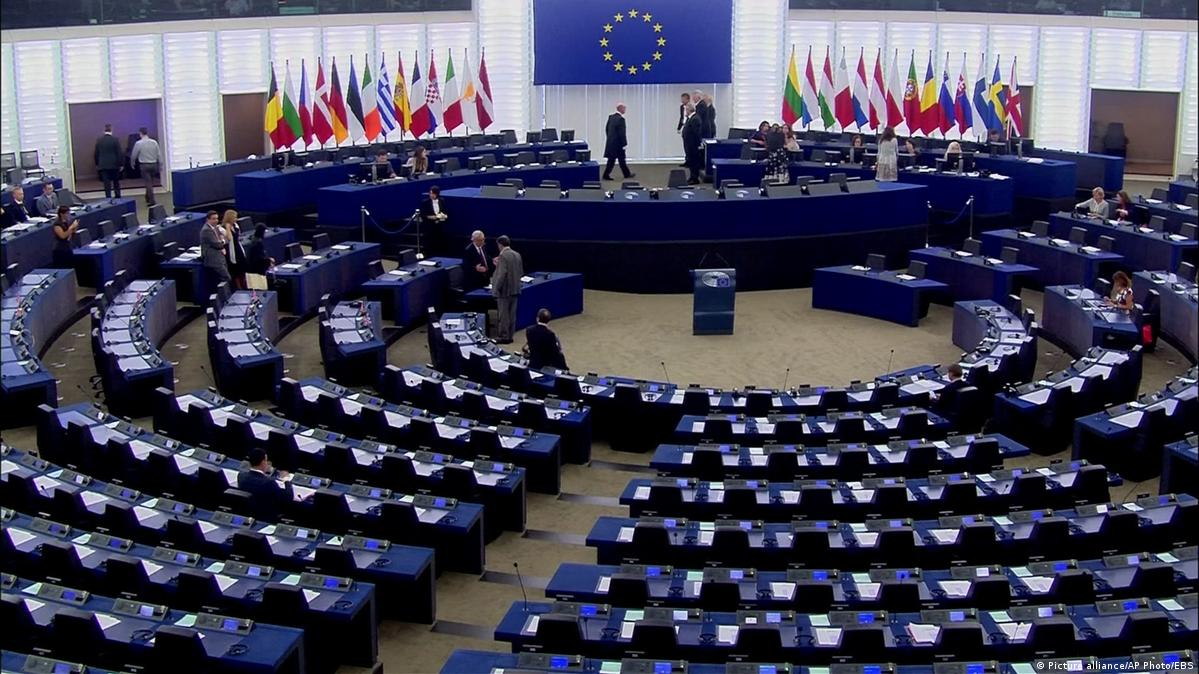
\includegraphics[width=\paperwidth,height=\paperheight,keepaspectratio]{img/euparl.jpg}}

\begin{document}
\begin{frame}[plain]
    \maketitle
\end{frame}

\begin{frame}{Introduction}
	
	\begin{figure}
		The European Parliament
	
		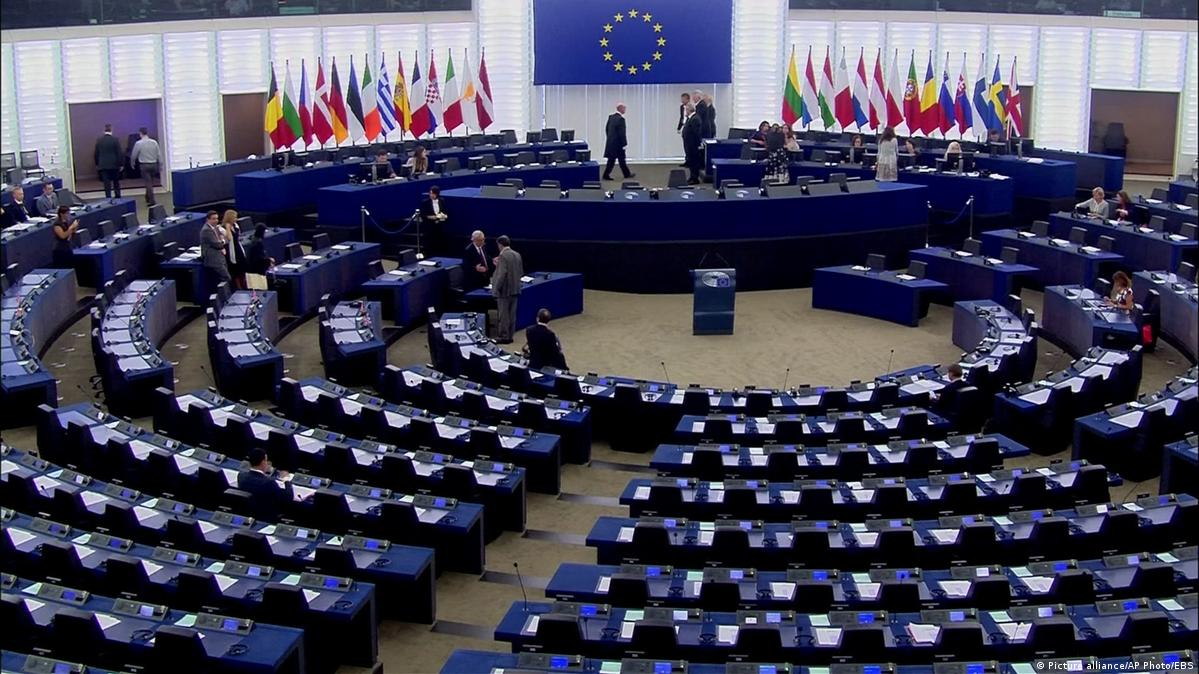
\includegraphics[width=0.5\textwidth]{img/euparl.jpg}
	\end{figure}

	We are analyzing a dataset of European Parliament members.
	
	\vspace{2mm}
	
	Our dataset is a list of 

	
\end{frame}

\begin{frame}{Analysis topic}
	
	We want to analyze the changes in the social network of the EP over time.
	
	\vspace{2mm}
	
	\pause For this, we picked two important properties of the network to investigate\begin{itemize}
		\pause \item Centrality of MEPs
		
		\pause \item Cohesion of the network
	\end{itemize}
	
\end{frame}

\begin{frame}{Analyzing centrality in the network}
	
	TODO
	
\end{frame}

\begin{frame}{Analyzing centrality in the network}
	
	TODO
	
\end{frame}

\begin{frame}{Analyzing the cohesion of the network}
	
	Cohesion: a measure of how well-connected a network is
	
	\vspace{2mm}
	
	\pause We will measure the cohesion of certain subgraphs of the MEP social network
	
	\vspace{2mm}
	
	\pause Our measure of cohesion is that we find the proportion of edges that are present -- i.e. the proportion of MEP-pairs that worked together
	
	\pause \[
		\text{cohesion} = \frac{\#\text{edges}}{\binom{n}{2}}
	\]
	
\end{frame}

\begin{frame}{Analyzing the cohesion of the network}
	
	Question: which subgraphs to consider?
	
	\vspace{2mm}
	
	\pause We want to analyze the changes in cohesion over time: for example the cohesion of specific parties
	
	\vspace{2mm}
	
	\pause We make use of the `committee' system of the EP to achieve this:
	
	\vspace{2mm}
	
	\pause Commitee members work together on a specific set of law changes
	
	\vspace{2mm}
	
	\pause We will analyze the changes in cohesion based on the committees
	
\end{frame}

\begin{frame}{}
	
	thx for watching
	
\end{frame}


\end{document}
